%************************************************
\chapter[Appendix 2.2: Chapter 2 - Adjacency matrices]{Appendix 2.2: Chapter 2 - Adjacency matrices and multilayer representations}\label{ch:Appendix2.2}
%************************************************
\renewcommand{\thefigure}{A.2.2.\arabic{figure}}
\setcounter{figure}{0}

\renewcommand{\thetable}{A.2.2.\arabic{table}}
\setcounter{table}{0}

Networks with static interaction strength coefficients can be represented consistently through adjacency matrices. Here we show, for the three frameworks presented, the adjacency matrices representing the Aire Island community. We also discuss alternative representations of ecological networks in the multilayer framework.

\section*{Expanded Food Webs}

In the formulation used, we modelled four ecological mechanisms: trophic interactions, nontrophic interactions that affect growth rate, and nontrophic interactions that affect mortality rate, as well as interaction modifiers. The three first mechanisms are represented by one adjacency matrix. Interaction modifiers represent the effect of one species on a given interaction, so that in a community of N species, N potential interaction modifiers matrices could exist. In the matrices (Fig. \ref{fig:figApp2.2.1}) we adhere to the definitions adopted in Chapter 2, in that we consider the feeding element of mutualisms as trophic interactions, while the subsequent benefits for the plant species are considered as non-trophic interactions.

\begin{figure}[ht]
\centering
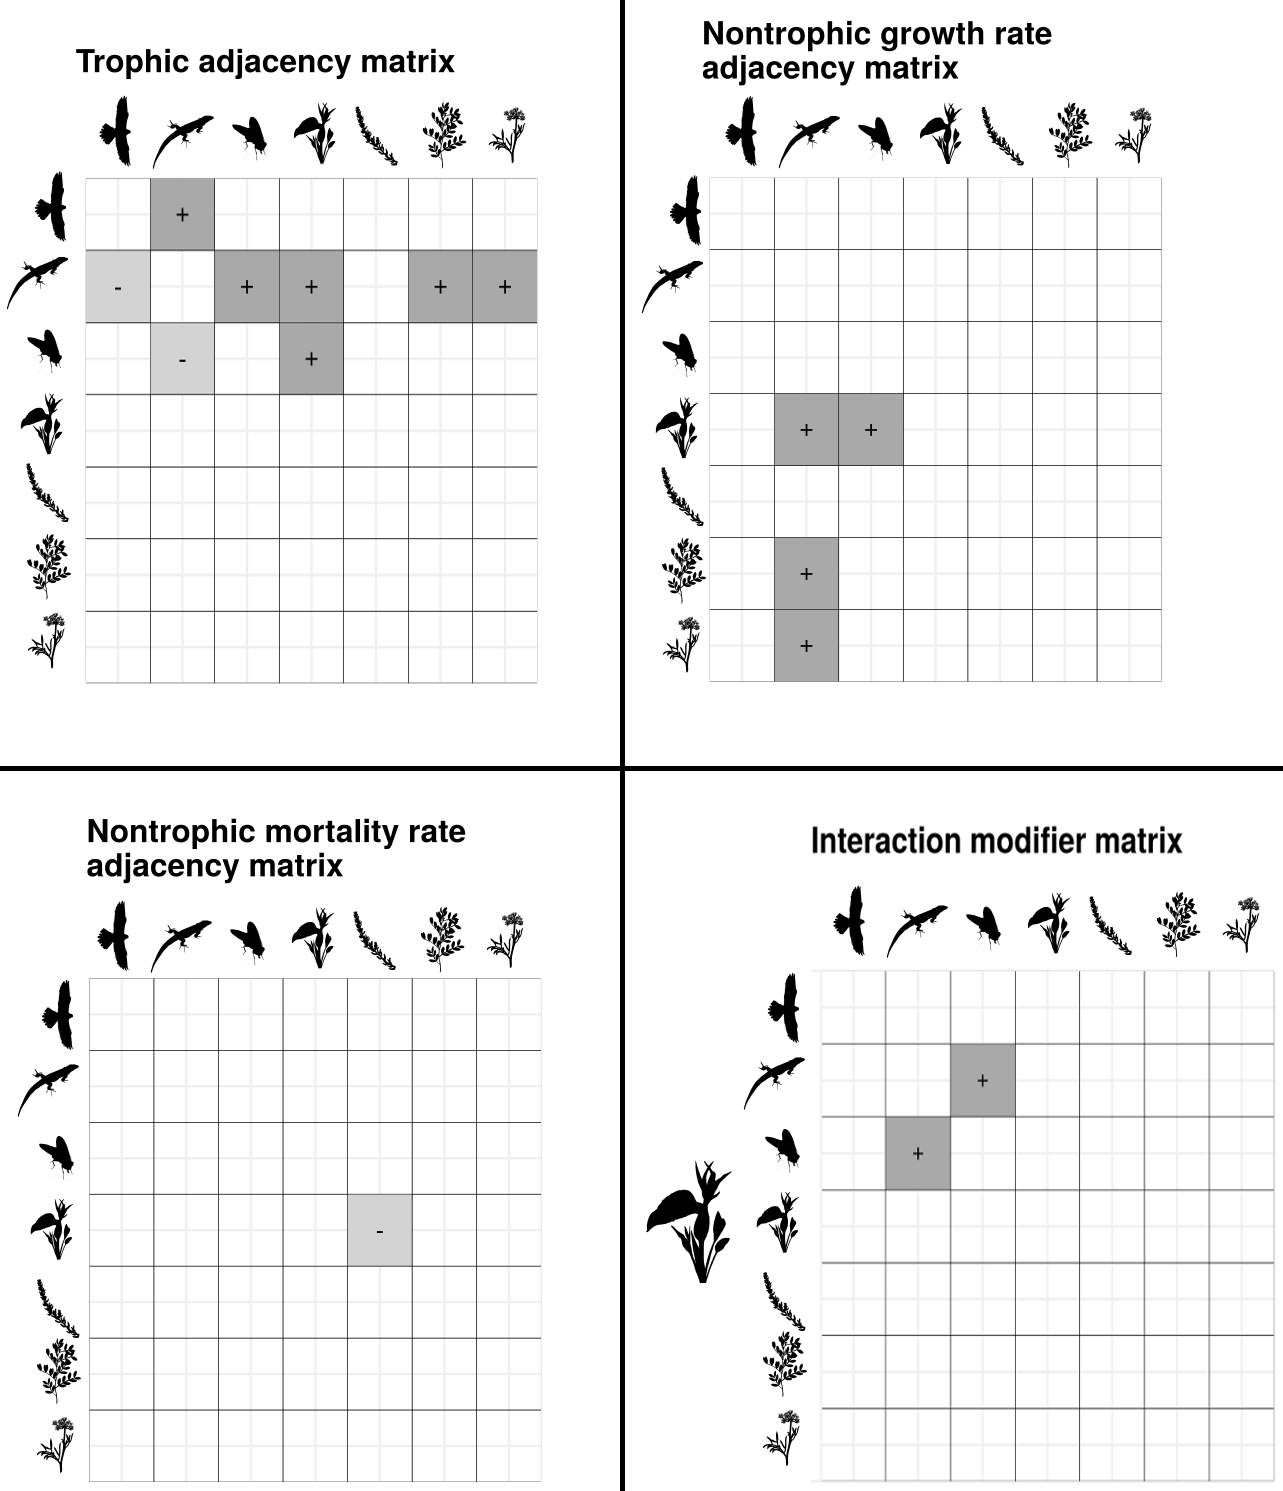
\includegraphics[width=.6\textwidth]{./Figures/Appendix2_2/ExFW_all.png}
\caption[Expanded Food Web Matrices]{\color{Gray} Adjacency matrices of the Expanded food web of the Aire Island community. In the trophic adjacency matrix, signs indicate effects of species in columns over species in rows. In the nontrophic matrices, signs indicate the effect of species in columns over the growth and mortality rates of the species in rows, respectively. In the interaction modifier matrix, the whole matrix represents the effects of Helicodiceros muscivorus (leftmost silhouette) over the community trophic interactions. The positive signs indicate that the presence of the dead horse arum increases the absolute magnitude of the Podarcis lilfordi – Diptera interaction. As this is the only interaction modifier considered in the community, the other six interaction modifier matrices are not shown.}
\label{fig:figApp2.2.1}
\end{figure}

\section*{Multilayer Networks}

\subsection*{Representing multiple interaction types with multilayer networks}

Due to the flexibility of the multilayer framework, it is often possible to design representations of the same network with different layering dimensions (see section 2.4 of \cite{Kivela2014}, where they frame the discussion in terms of node-coloured and edge-coloured graphs). In the context of ecological networks with different interaction types, different layers usually represent different interaction types, but another option is to separate layers by taxonomic groups, so that intra-layer links represent these within a given guild and inter-layer links are between-guild interactions (Fig. \ref{fig:figApp2.2.2}, cf. \cref{fig:fig2.2}). In the first representation, emphasis is given to the sub-networks of different interaction types, and their structure and dynamics can be tracked separatedly. In the second one, the guild structure of the community is the priority, and it is a natural representation for analyzing patterns of interactions of the different guilds or differences in within-guild and between-guild interactions. In terms of network structure, the first representation is potentially node-aligned, i.e. all nodes can appear in all layers, and there is at least one intra-layer link for each layer. The second representation, however, is layer-disjoint, i.e. a node exists at most in one layer, and there can exist layers without any intra-layer links. In that sense, thus, the guild representation does not connect subnetworks, but sets of entities. We have found no explicit examples of the guild representation in ecological studies, but empirical datasets such as the one compiled by \citep{Pocock2012} can be looked at in both ways of representation.

\begin{figure}[ht]
\centering
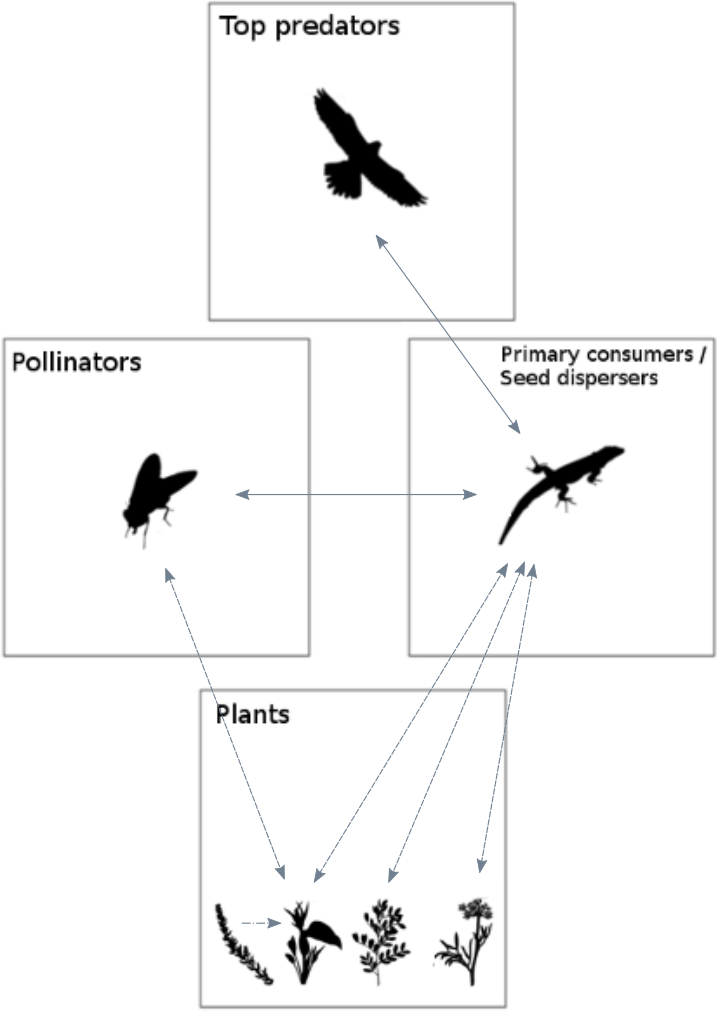
\includegraphics[width=.5\textwidth]{./Figures/Appendix2_2/MLN_alternative.png}
\caption[Multilayer functional guilds]{\color{Gray} A multilayer representation of the Aire Island community where layers represent functional guilds. Note how in this representation, only one intra-layer link exists, that of the commensalist relationship between \textit{Suaeda vera} and \textit{Helicodiceros muscivorus}. In each interaction, an arrow tip indicates a non-neutral effect over a species.}
\label{fig:figApp2.2.2}
\end{figure}

\subsection*{Adjacency matrices of multiplex networks}

Multilayer networks can be represented consistently as $rank-2(d + 1)$ adjacency tensors, where $d$ is the number of aspects or dimensions of the network \citep{Kivela2014}. The tensorial representation is only valid for node-aligned networks, i.e. networks in which all nodes are represented in all layers. While this constraint can be relaxed (see \citealt{Kivela2014} for details), multilayer networks can also be represented through so-called supra-adjacency matrices, whereby one loses some information about the aspects (due to the ``flattening'' of the network) but one can represent networks that are not node-aligned and, importantly, use standard matrix algebra to analyze network structure. These supra-adjacency matrices represent in the same structure the three types of links potentially present in multilayer networks: intra-layer links in the diagonal blocks, coupling links in the diagonal elements of the off-diagonal blocks, and inter-layer links in the off-diagonal elements of the off-diagonal blocks (Fig. \ref{fig:figApp2.2.3}). The distinction between coupling and inter-layer links is that coupling links are connecting the same node in different layers, while inter-layer links connect different nodes in different layers. The Aire Island multilayer network, where each layer is an interaction type, is not node-aligned (i.e. not all nodes are present in all layers), hence the supra-adjacency matrix is not square and not all coupling links are realized (Fig. \ref{fig:figApp2.2.4}).

\begin{figure}[ht]
\centering
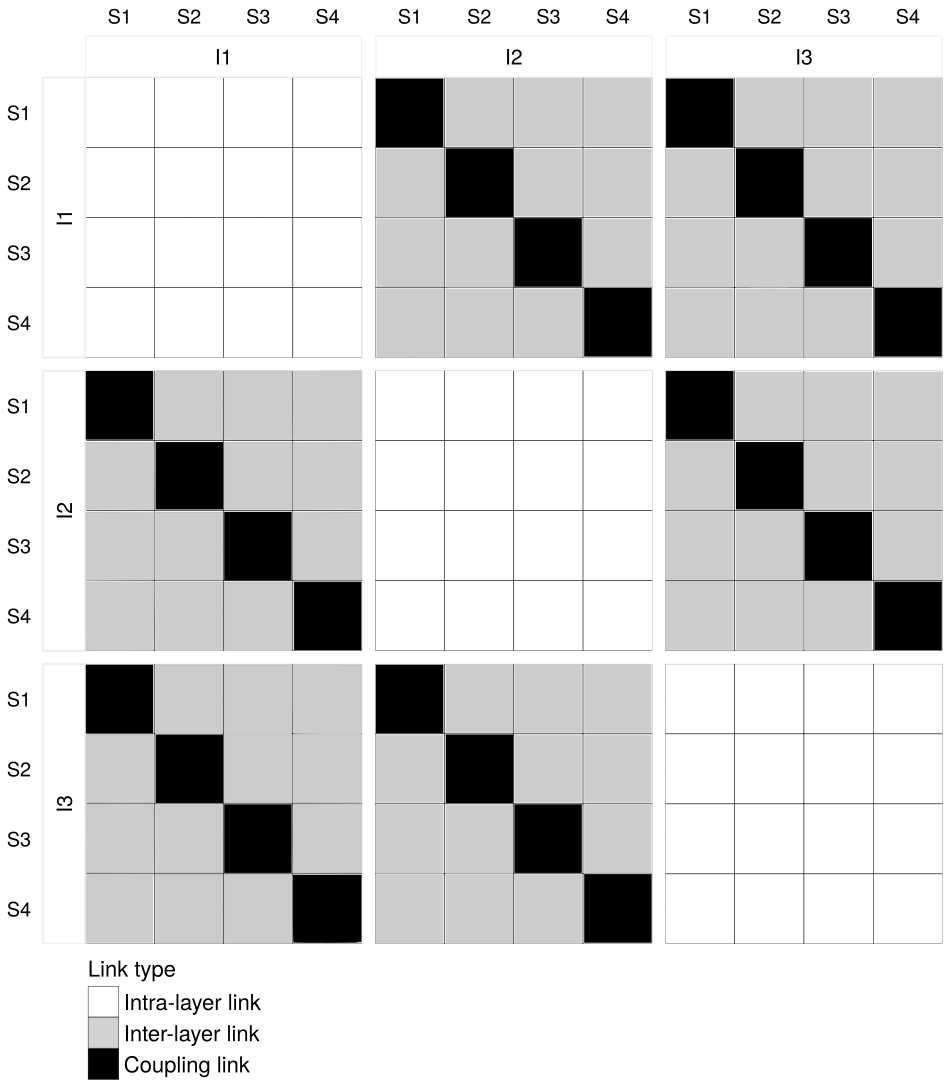
\includegraphics[width=.5\textwidth]{./Figures/Appendix2_2/MLN_supra_adjacency_example.png}
\caption[Multilayer supra adjacency matrix]{\color{Gray} An example of supra-adjacency matrix showing the placement of intra-layer, coupling and inter-layer links. In this setting, the network consists of four nodes (S1-S4) interacting in three different ways (I1-I3). All four species are represented in the three sub-networks, so that the network is node-aligned. Blocks are slightly separated for visibility}
\label{fig:figApp2.2.3}
\end{figure}

\begin{figure}[ht]
\centering
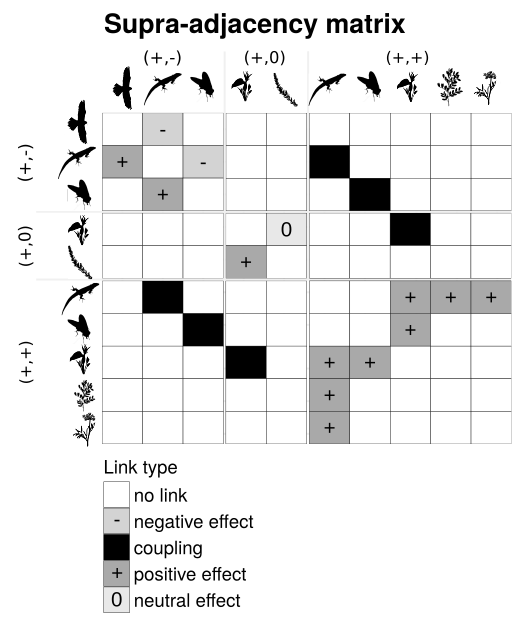
\includegraphics[width=.6\textwidth]{./Figures/Appendix2_2/MLN_supra_adjacency_AIRE.png}
\caption[Multilayer supra adjacency Aire island]{\color{Gray} Supra-adjacency matrix of the Aire Island multilayer network. The (+,-) block represents the antagonist subnetwork, (+,0) the commensalist one and (+,+) the mutualist one.}
\label{fig:figApp2.2.4}
\end{figure}
